\documentclass[12pt,a4paper]{article}
\usepackage[utf8]{inputenc}
\usepackage[english]{babel}
\usepackage{amsmath}
\usepackage{amsfonts}
\usepackage{amssymb}
\usepackage{graphicx}
\usepackage[left=2cm,right=2cm,top=2cm,bottom=2cm]{geometry}
\begin{document}

\raggedright

\section*{Questionnaire 1}

\begin{enumerate}
\item Do you need these for deep learning?
\begin{itemize}
	\item Lots of math T / \textbf{F}
	\item Lots of data T / \textbf{F}
	\item Lots of expensive computers T / \textbf{F}
	\item A PhD T / \textbf{F}
\end{itemize}

\item Name five areas where deep learning is now the best in the world. \\

\begin{enumerate}
	\item natural language processing
	\item computer vision
	\item medicine and biology
	\item image generation
	\item recommendation systems
\end{enumerate}

\item What was the name of the first device that was based on the principle of the artificial neuron? \\

\smallbreak

Mark I Perceptron

\bigbreak

\item Based on the book of the same name, what are the requirements for parallel distributed processing (PDP)? \\

\begin{itemize}
	\item[1.] a set of \textit{processsing units}
	\item[2.] a \textit{state of activation}
	\item[3.] an \textit{output function} for each unit
	\item[4.] a \textit{pattern of connectivity} among units
	\item[5.] a \textit{propagation rule} for propagating patterns of activities through the network of connectivities
	\item[6.] an \textit{activation rule} for combining the inputs impinging on a unit with the current state of that unit to produce an output for the unit
	\item[7.] a \textit{learning rule} whereby patterns of connectivity are modified by experience
	\item[8.] an \textit{environment} within which the system must operate
\end{itemize}

\item What were the two theoretical misunderstandings that held back the field of neural networks? \\

\smallbreak

Marvin Minsky and Seymour Papert wrote a book called \textit{Perceptrons}, where they showed a single layer of neural nodes were unable to learn some simple but critical mathematical functions (such as XOR). In theory, adding just one extra layer of neurons was enough to allow any mathematical function to be approximated with these neural networks, but in practice (back then) such networks were often too big and too slow to be useful.

\bigbreak

\item What is a GPU? \\

\smallbreak

A graphics processing unit (GPU) is a special kind of processor that can perform multiple (thousands) of tasks at a time, especially designed for displaying 3D environments in video games.

\bigbreak

\item Open a notebook and execute a cell containing: 1+1. What happens? \\

\smallbreak

In a Jupyter Notebook, executing 1+1 will output 2.

\bigbreak

\item Why is it hard to use a traditional computer program to recognize images in a photo? \\

\smallbreak

The computer doesn't know what to look for to recognize what objects are in an image. In general, for a computer program, we give it a list of instructions based roughly on how a human would do so, but it is hard to write down instructions for a computer to recognize objects since we ourselves aren't sure of the process; our brain automatically recognizes things.

\bigbreak

\item What did Samuel mean by "weight assignment"? \\

\smallbreak

Weights are just variables, and a weight assignment is a particular choice of values for those variables.

\bigbreak

\item What term do we normally use in deep learning for what Samuel called "weights"? \\

\smallbreak

Parameters.

\bigbreak

\item Draw a picture that summarizes Samuel's view of a machine learning model. \\

\smallbreak

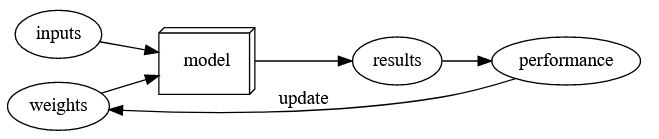
\includegraphics[scale=1]{model.jpeg}

\bigbreak

\item Why is it hard to understand why a deep learning model makes a particular prediction? \\

\smallbreak

Think of a deep learning model as a human brain in a way. There are many processes that go into us formulating a thought or classifying an animal as a cat or a dog. Deep neural networks have thousands of layers of neurons. It is hard to determine what factors went into determining the final output and how important each factor was. Each layer of the network interact with each other, with each layer feeding to other layers. Because of the complex nature of deep learning models, it is very difficult why a neural network outputs a given prediction.

\bigbreak

\item What is the name of the theorem that shows that a neural network can solve any mathematical problem to any level of accuracy? \\

\smallbreak

The \textbf{universal approximation theorem} states that neural networks can theoretically represent any mathematical function. However, because of the limitations of available data and computer hardware, it is practically impossible to do so.

\newpage

\item What do you need in order to train a model? \\

\smallbreak

You will need an architecture (the functional form of the model) for your given task or problem along with data to feed in as input. Most cases will require labels for your data so that you can compare your predictions and see how accurate your model is (using a loss function). Using your loss function, you need a way to be able to update your parameters in order to improve its performance.

\bigbreak

\item How could a feedback loop impact the rollout of a predictive policing model? \\

\smallbreak

In a predictive policing model, a positive feedback loop may occur, leading to a highly biased model with little predictive power. The model is created using data on previous arrests. The model is not actually predicting crime, but rather predicting arrests, and is therefore partially biased on current policing policies. Officers may then use that data to determine the areas that need the most enforcement, resulting in more arrests in those locations. Data on those additional arrests are passed into the model for future versions to be trained on, thus creating a positive feedback loop.

\bigbreak

\item Do we always have to use 224×224-pixel images with the cat recognition model? \\

\smallbreak

No. 224x244 was used for historical reasons, but it is not required nowadays. You can increase the size for better performance at the cost of speed and consumption and vice versa.

\bigbreak

\item What is the difference between classification and regression? \\

\smallbreak

Classification is focused on predicting a class or category (ex: a type of pet). Regression is focused on predicting a numeric quantity (ex: price of house).

\bigbreak

\item What is a validation set? What is a test set? Why do we need them? \\

\smallbreak

A validation set is the portion of the dataset that is not used for training and is instead use for evaluating the model during training in order to prevent overfitting. This ensures the model is not just memorizing the dataset. \\
\smallbreak
However, it is possible that we overfit the validation set as well. This is the because the human interpreter is also part of the training process, adjusting hyperparameters and training procedures according to the validation performance. Therefore, another unseen portion of the dataset, called the test set, is used for the final evaluation of the model. The splitting of the dataset is necessary to ensure that the model generalizes to unseen data.

\bigbreak

\item What will fastai do if you don't provide a validation set? \\

\smallbreak

It will automatically provide a validation set that is by default set to 20\% of the dataset, randomly chosen.

\bigbreak

\item Can we always use a random sample for a validation set? Why or why not? \\

\smallbreak

Not always. A good validation or test set should be representative of future data that you may encounter, and a random sample might not be the best choice. For example, for time series data, selecting random samples doesn't make sense.

\bigbreak

\item What is overfitting? Provide an example. \\

\smallbreak

Overfitting refers to when a model fits too closely to a limited set of data but does not generalize well to unseen data. This will happen if a neural network trains too much on one set of training data, as it will potentially start to "memorize" the given data and fail to generalize for all unseen data.

\bigbreak

\item What is a metric? How does it differ from "loss"? \\

\smallbreak

A metric is a function that measures quality of the model's predictions using the validation set. This is similar to "loss," which is also a measure of performance of the model. However, loss is meant for the optimization algorithm (like SGD) to efficiently update the model parameters, while metrics are are human-interpretable measures of performance. 

\bigbreak

\item How can pretrained models help? \\

\smallbreak

Pretrained models have been trained on other problems that may be quite similar to the current task. They are useful because they have already learned how to handle a lot of simple features like edge and color detection. However, since the model was trained for a different task than already used, it cannot be used as is.

\bigbreak

\item What is the "head" of a model? \\

\smallbreak

When using a pretrained model, the later layers of a model, which were useful for the task that the model was originally trained on, are replaced with one or more new layers with randomized weights, of an appropriate size for the dataset you are currently working on. These new layers are called the "head" of the model.

\bigbreak

\item What kinds of features do the early layers of a CNN find? How about the later layers? \\

\smallbreak

Earlier layers of a CNN learn features such as edges. Later layers learn more specialized features like car wheels, flower petals, and outlines of objects.

\bigbreak

\item Are image models only useful for photos? \\

\smallbreak

No. Image models are useful on other types of images like sketches, medical data, etc. \\
\smallbreak
A lot of information can be represented as images, even when there seems to be no correlation between them and images. For example, sound can be converted into a spectrogram, which is a visual representation of the audio. Time series data can also be plotted on a graph, therefore converting the data into an image.

\bigbreak

\item What is an "architecture"? \\

\smallbreak

The architecture is the template or structure of the model we are trying to fit. It defines the mathematical model we are trying to fit.

\bigbreak

\item What is segmentation? \\

\smallbreak

Segmentation is a pixelwise classification problem. We attempt to predict a label for every single pixel in the image. This provides a mask for which parts of the image correspond to the given label.

\bigbreak

\item What is y\_range used for? When do we need it? \\

\smallbreak

y\_range is used to limit the values predicted when our problem is focused on predicting a numeric value in a given range (ex: predicting movie ratings, range of 0.5-5.5).

\bigbreak

\item What are "hyperparameters"? \\

\smallbreak

Training models requires various other parameters that define \textit{how} the model is trained. For example, we need to define how long we train for, or what learning rate (how fast the model parameters are allowed to change) is used. These sorts of parameters are hyperparameters.

\bigbreak

\item What's the best way to avoid failures when using AI in an organization? \\

\begin{enumerate}
\item Make sure a training, validation, and test set is properly defined in order to evaluate the model in an appropriate manner. \\
\item Try out a simple baseline, which future models should hopefully beat. This baseline may even be enough at times. \\
\end{enumerate}

\end{enumerate}

\section*{Further Research}

\begin{enumerate}

\item Why is a GPU useful for deep learning? How is a CPU different, and why is it less effective for deep learning? \\

\smallbreak

GPUs can process thousands of things at one time because of its high number of cores. Compared to CPUs, GPUs have higher bandwidth ( more quantity of things can be transferred), higher thread parallelism (more processes at one time), and easily programmable registers.

\bigbreak

\item Try to think of three areas where feedback loops might impact the use of machine learning. See if you can find documented examples of that happening in practice.

\smallbreak

Look back to the feedback loop for an example to this.
\end{enumerate}

\end{document}